% ============================================================
%  N.2.7  Eyeriss CS6: Per-Block Fusion Overhead
% ============================================================
\subsection{Eyeriss: Per-Block Fusion Overhead (CS6)}
\label{sec:eyeriss-cs6}

\subsubsection{Motivation}

The previous case studies (CS1--CS5) varied architecture parameters
while keeping the fused workload fixed.
CS6 addresses a complementary question:
\emph{what is the actual cost of fusing a single pair of consecutive
layers, compared with executing the same layers independently?}

The preceding fusion comparisons (Section~\ref{sec:fusion-comp})
aggregate \emph{all} partial blocks and all single layers into two
sums, which masks per-block variation.
Here we isolate the \textbf{earliest fused block} of VGG16 and
ResNet18---the two weight-dominant workloads---and compare its
energy, latency, and EDP against the sum of the two constituent
single-layer executions on the same architecture.

The earliest block is the most challenging for fusion because it
operates on the largest spatial dimensions.
Large activation maps force small tile sizes in the fused mapping,
which in turn requires more temporal iterations and drives up weight
re-reads through the memory hierarchy.

\subsubsection{Setup}

We use the Eyeriss $512 \times 32$ array with $\text{GB} = 128$\,KB,
$\text{InReg} = 400$, $\text{IntReg} = 350$, $\text{OutReg} = 64$
entries, and $\text{DRAM} = 160$\,pJ/byte.
For VGG16 we set $\text{WReg} = 576$; for ResNet18
$\text{WReg} = 384$.

The two blocks under study are:
\begin{itemize}
  \item \textbf{VGG16 \texttt{block1}}: \texttt{conv1\_1} (L0) +
    \texttt{conv1\_2} (L1), operating at $224 \times 224$ spatial
    resolution with $3 \times 3$ kernels and output channels
    $64 \to 64$.
  \item \textbf{ResNet18 \texttt{s1b1}}: \texttt{conv1} (L0) +
    \texttt{conv2\_1\_1} (L1), with a $7 \times 7$ first kernel
    (stride~2) followed by a $3 \times 3$ second kernel at
    $56 \times 56$ resolution, both producing 64 output channels.
\end{itemize}

For each workload we report three quantities:
(i)~the metrics of the fused block, and
(ii)~the sum of the two corresponding single-layer runs, on the
identical architecture.

\subsubsection{Results}

Table~\ref{tab:eyeriss-cs6} summarises the comparison.

\begin{table}[htbp]
  \centering
  \caption{Eyeriss CS6: earliest fused block vs.\ sum of constituent
    single-layer executions.
    Ratio~$> 1$ means fusion is \emph{worse}.}
  \label{tab:eyeriss-cs6}
  \begin{tabular}{ll rrr}
    \toprule
    Workload & Mode & Energy ($\mu$J) & Latency (cc) & EDP \\
    \midrule
    \multirow{3}{*}{VGG16}
      & Fused block1       & $1.173 \times 10^{4}$ & $1.032 \times 10^{6}$
        & $1.34 \times 10^{4}$ \\
      & $\Sigma$ Singles    & $3.079 \times 10^{3}$ & $1.615 \times 10^{6}$
        & $4.97 \times 10^{3}$ \\
      & \textbf{Ratio}     & \textbf{3.81$\times$} & \textbf{0.64$\times$}
        & \textbf{2.70$\times$} \\
    \midrule
    \multirow{3}{*}{ResNet18}
      & Fused s1b1          & $1.547 \times 10^{3}$ & $1.380 \times 10^{5}$
        & $2.24 \times 10^{2}$ \\
      & $\Sigma$ Singles     & $3.360 \times 10^{2}$ & $2.601 \times 10^{5}$
        & $8.74 \times 10^{1}$ \\
      & \textbf{Ratio}      & \textbf{4.61$\times$} & \textbf{0.53$\times$}
        & \textbf{2.56$\times$} \\
    \bottomrule
  \end{tabular}
\end{table}

\paragraph{Energy.}
Fusion increases energy by $3.81 \times$ for VGG16 and
$4.61 \times$ for ResNet18.
The merged loop nest constrains the mapper: both layers share a
single spatial factorisation, and the intermediate activations must
fit in the register file or the global buffer at each tile iteration.
With the large spatial dimensions of these early layers
($224 \times 224$ for VGG16, up to $112 \times 112$ for ResNet18),
the tile size imposed by the fusion is small relative to the total
workload.
Each spatial tile therefore re-reads both layers' weights from the
global buffer or DRAM, amplifying weight-related energy far beyond
the single-layer optimum.

\paragraph{Latency.}
Fusion reduces latency by $36\%$ for VGG16 and $47\%$ for ResNet18.
The saving stems from eliminating the DRAM write of L0's output
activations and the DRAM read of L1's input activations: by keeping
the intermediate tensor on chip, the fused schedule avoids two full
DRAM passes.
For ResNet18 s1b1, the first layer's $7 \times 7$ kernel produces a
large intermediate map that would otherwise require substantial DRAM
bandwidth; removing that transfer yields the larger latency benefit.

\paragraph{EDP.}
Despite the latency improvement, the energy overhead dominates, and
the net EDP is $2.70 \times$ worse for VGG16 and $2.56 \times$ worse
for ResNet18.
The energy penalty roughly squares the latency benefit, leaving EDP
decisively in favour of the single-layer baseline.

\begin{figure}[htbp]
  \centering
  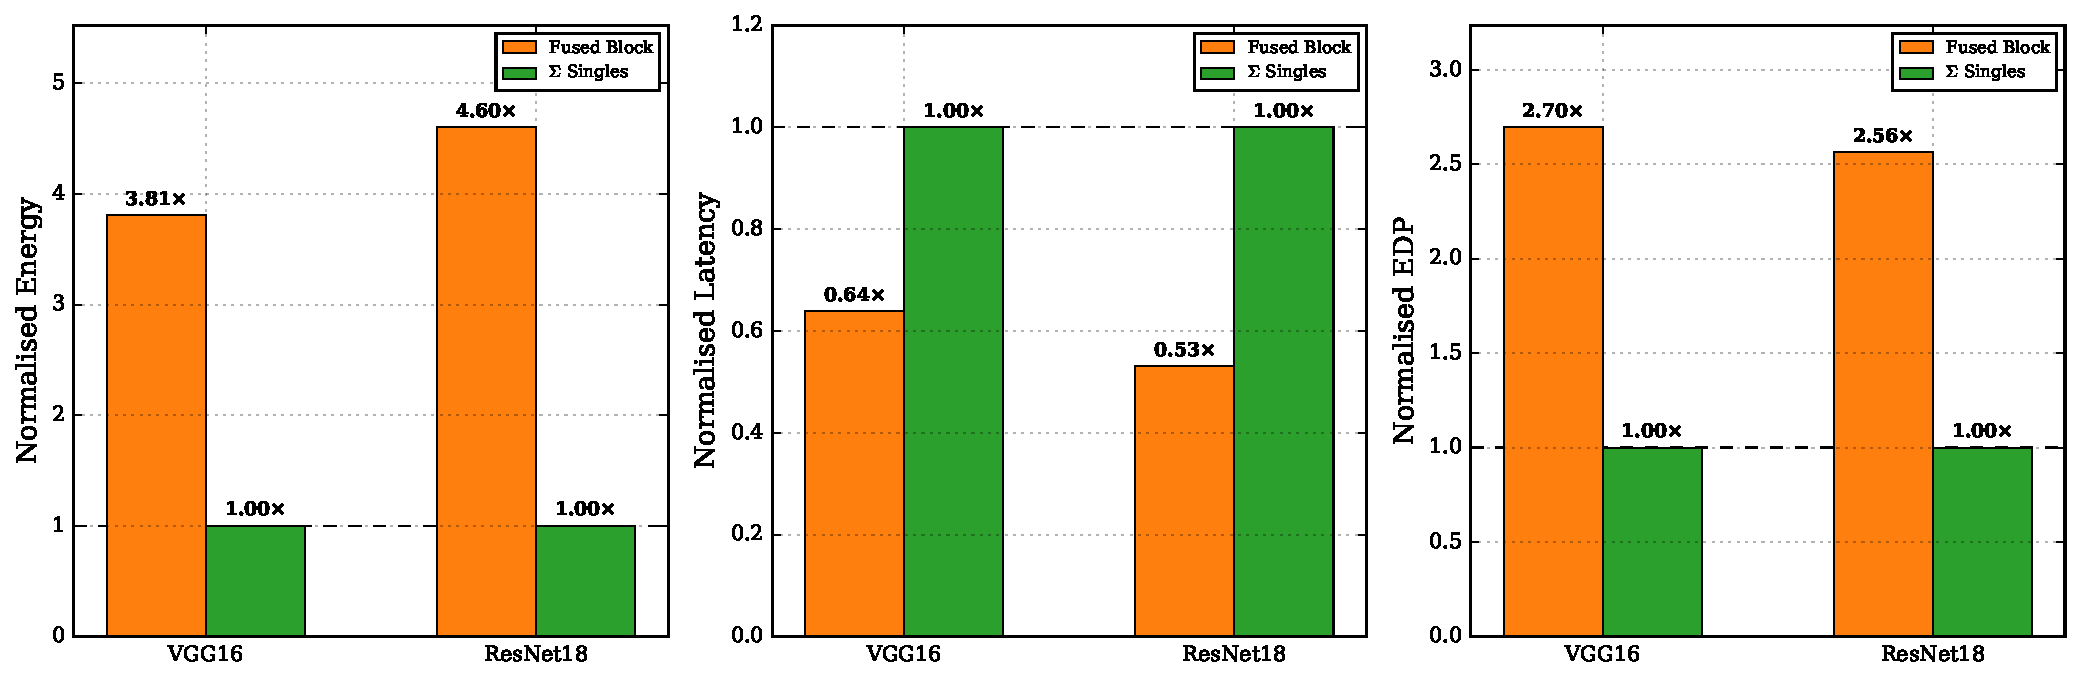
\includegraphics[width=0.85\textwidth]{plots/eyeriss_cs6_block_vs_singles.pdf}
  \caption{Eyeriss CS6: normalised energy, latency, and EDP of the
    earliest fused block relative to the sum of its constituent
    single-layer runs ($\Sigma$~Singles~$= 1.0$).}
  \label{fig:eyeriss-cs6}
\end{figure}

\paragraph{Considerations.}
For weight-dominant workloads at the earliest (largest spatial)
block, the mapping constraints imposed by layer fusion outweigh
the DRAM savings on intermediate activations.
Weights dominate the total data movement in these workloads, so the
eliminated intermediate traffic is a small fraction of the whole;
meanwhile, the restricted loop nest forces repeated weight re-reads
that inflate energy by almost $4\text{--}5 \times$.

This result complements the aggregate fusion comparisons presented in
Section~\ref{sec:fusion-comp}: while the sum across all blocks shows
the overall fusion overhead, CS6 reveals that the penalty is
concentrated in the earliest blocks, where spatial dimensions are
largest and the fusion constraints are most restrictive.
Deeper blocks, with smaller activation maps and fewer tiling
iterations, are expected to suffer a milder overhead.
A practical fusion strategy could therefore skip the earliest blocks
and apply fusion only to the deeper stages of the network,
selectively trading a small latency benefit for a much larger energy
saving.
